\problem{Anomalie de Schottky \cite{Tremblay}}

\question{Sans calcul explicite, faites un graphique qualitatif de l’énergie moyenne du système à deux niveaux en fonction de sa température en expliquant physiquement votre résultat. Près de quelle
température l’énergie change-t-elle de sa valeur minimale à sa valeur limite haute température ?}
Nous savons qu'à basse température, l'énergie de la source est $\epsilon_1$. Aussi, nous savons qu'à haute température, l'énergie de la source est de $\epsilon_2$. Nous avons une fonction qui part à $\epsilon_1$ et qui va jusqu'à 
$\epsilon_2$, avec une transition tel que représentée dans le graphique suivant.
\begin{figure}[!ht]
        \centering
        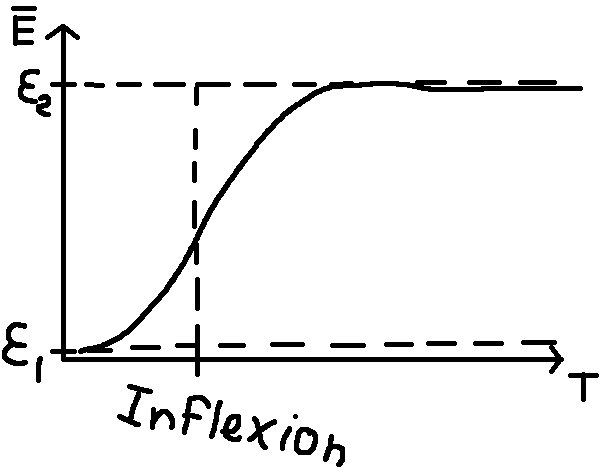
\includegraphics[scale= 0.6 ]{figs/3_a.png}
       \caption{Variation de l'énergie moyenne d'un système à deux niveaux selon la température.}
        \label{fig: a}
\end{figure}
Le moment où il y a un changement d'énergie correspond au point d'inflexion du graphique.

\question{Utilisant le résultat de a, faites un graphique qualitatif de la chaleur spécifique à volume
constant en fonction de la température.}
Nous savons que $C_V = \dv{\bar{E}}{T}$, où $\bar{E}$ est la valeur moyenne de l'énergie. À partir du graphique précédent, nous pouvons tracer le graphique suivant.
\begin{figure}[!ht]
        \centering
        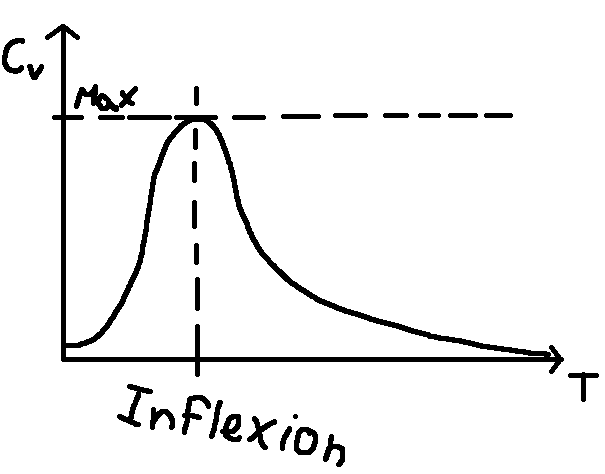
\includegraphics[scale= 0.6 ]{figs/3_b.png}
       \caption{Variation de la chaleur spécifique d'un système à deux niveaux selon la température.}
        \label{fig: b}
\end{figure}
Puisque ce graphique est la dérivée du graphique précédent, nous avons que le point d'inflexion du graphique(\ref{fig: a}) est le maximum du graphique(\ref{fig: b}), soit la valeur maximum de $C_V$.
\\ \\ \\ \\ \\ \\ \\
\question{Calculez explicitement l’énergie moyenne et la chaleur spécifique CV (T ) de ce système à l’aide
de la fonction de partition.}
D'abord, nous avons que $Z = e^{-\beta \epsilon_1} + e^{-\beta \epsilon_2} = e^{-\beta \epsilon_2}\qty(e^{\beta \Delta \epsilon} +1)$, soit la somme sur toutes les valeurs d'énergie. 
Nous pouvons exprimmer la valeur moyenne de l'énergie $(\bar{E})$ comme :
\[
        \bar{E} &= -\pdv{ln\qty|Z|}{\beta} \notag \\
        &= \frac{-1}{e^{-\beta \epsilon_2}\qty(e^{\beta \Delta \epsilon} +1)} \qty(-\epsilon_2 e^{-\beta \epsilon_2}\qty[e^{\beta \Delta \epsilon} +1] + e^{-\beta \epsilon_2}\qty[\Delta \epsilon e^{\beta \Delta \epsilon}]) \notag \\
        &= \frac{\epsilon_2 \qty(e^{\beta \Delta \epsilon} +1) - \Delta \epsilon e^{\beta \Delta \epsilon}}{e^{\beta \Delta \epsilon} + 1} .\notag
\]
Nous avons donc la chaleur spécifique tel que $C_V = \dv{\bar{E}}{T} = \dv{\bar{E}}{\beta} \dv{\beta}{T} = \frac{-1}{k_B T^2} \dv{\bar{E}}{\beta}$. Nous pouvons donc calculer $\dv{\bar{E}}{\beta}$ :
\[
        \dv{\bar{E}}{\beta} &= \frac{e^{\beta \Delta \epsilon} \qty[\epsilon_2 \Delta \epsilon - (\Delta \epsilon)^2]\qty(e^{\beta \Delta \epsilon} + 1) - \Delta \epsilon e^{\beta \Delta \epsilon} \qty[\epsilon_2\qty(e^{\beta \Delta \epsilon} + 1) - \Delta \epsilon e^{\beta \Delta \epsilon}]}{\qty(e^{\beta \Delta \epsilon} + 1)^2} \notag \\
        &= \frac{e^{\beta \Delta \epsilon} \qty(\epsilon_2 \Delta \epsilon e^{\beta \Delta \epsilon} + \epsilon_2 \Delta \epsilon - \epsilon_2 \Delta \epsilon - \epsilon_2 \Delta \epsilon e^{\beta \Delta \epsilon} - (\Delta \epsilon)^2 e^{\beta \Delta \epsilon} - (\Delta \epsilon)^2 + (\Delta \epsilon)^2 e^{\beta \Delta \epsilon})}{\qty(e^{\beta \Delta \epsilon} + 1)^2} \notag \\
        &= \frac{e^{\beta \Delta \epsilon} \qty(- (\Delta \epsilon)^2 e^{\beta \Delta \epsilon} - (\Delta \epsilon)^2 + (\Delta \epsilon)^2 e^{\beta \Delta \epsilon})}{\qty(e^{\beta \Delta \epsilon} + 1)^2} \notag \\
        &= \frac{(\Delta \epsilon)^2 e^{\beta \Delta \epsilon} \qty(-1)}{\qty(e^{\beta \Delta \epsilon} + 1)^2} \notag \\
        &= \frac{-(\Delta \epsilon)^2 e^{\beta \Delta \epsilon}}{\qty(e^{\beta \Delta \epsilon} + 1)^2} .\notag
\]
Nous avons donc :
\[
      C_V &= \frac{-1}{k_B T^2} \frac{-(\Delta \epsilon)^2 e^{\beta \Delta \epsilon}}{\qty(e^{\beta \Delta \epsilon} + 1)^2} \notag \\
      &= \frac{1}{k_B T^2} \frac{(\Delta \epsilon)^2 e^{\beta \Delta \epsilon}}{\qty(e^{\beta \Delta \epsilon} + 1)^2} .\notag
\]
\clearpage
